\documentclass{article}
\usepackage[centering]{geometry}
\usepackage[T1]{fontenc}
\usepackage[utf8]{inputenc} % Ensure proper encoding
\usepackage{lmodern} % Use Latin Modern fonts which provide more sizes
\usepackage{babel}

%----- Math ---------------------------------------------
\usepackage{amsmath}         
\usepackage{mathtools}       
\usepackage{amssymb}   
\usepackage{amsthm}         

%----- Design ------------------------------------------- 
\usepackage{lastpage}                              
\usepackage{enumitem}
%----- Pacchetti Disegno --------------------------------
\usepackage{tikz}
\usepackage{tikz-cd}
\usepackage{graphicx}
\usepackage{thmtools}
\usepackage{xcolor}
\usepackage[all]{xy}        
\usetikzlibrary{decorations.markings}
\usetikzlibrary{hobby}
\usepackage{pgfplots}
\pgfplotsset{compat=1.18}

%----- Symbols -----------------------------------------
\providecommand{\R}{\mathbb{R}}
\providecommand{\N}{\mathbb{N}}
\providecommand{\Z}{\mathbb{Z}}
\providecommand{\Sp}{\mathbb{S}}
\providecommand{\D}{\mathbb{D}}
\providecommand{\E}{\mathbb{E}}
\providecommand{\F}{\mathbb{F}}
\providecommand{\T}{\mathcal{T}}
\providecommand{\de}{\partial}
\providecommand{\ve}{\varepsilon}
\providecommand{\vphi}{\varphi}
\providecommand{\dif}{\mathrm{d}}
\providecommand{\integral}[3]{\int_{#1} #2 \mathrm{d}#3}
\providecommand{\id}{\mathrm{id}}
\providecommand{\sff}{\mathrm{I\!I}}
\newcommand{\mapsfrom}{\mathrel{\reflectbox{\ensuremath{\mapsto}}}}

%----- MathOperators -----------------------------------
\DeclareMathOperator{\grad}{grad}

\title{DISEGNI}
\author{Andrea Martelli}
\begin{document}
	Modelli1
	%MODELLI 1

\begin{figure}[h]
	\centering
	\begin{tikzpicture}
		%\draw [help lines] (-3,-4) grid (9,4);
		
		%SFERA
		%linee
		\draw [thick] (0,0) circle (2);
		\draw (-2,0) arc (180:360: 2 and 0.55);
		\draw [dashed] (2,0) arc (0:180: 2 and 0.55);
		
		
	
		
		%TORO
		%linee
		\draw[thick] (6,0) ellipse (2.5 and 1.5);
		\begin{scope}
			\clip (6,-1.8) ellipse (2.5 and 2.5);
			\draw[thick] (6,2.2) ellipse (2.5 and 2.5);
		\end{scope}
		\begin{scope}
			\clip(6,2.2) ellipse (2.5 and 2.5);
			\draw[thick] (6,-2.2) ellipse (2.5 and 2.5);
		\end{scope}
		
	\end{tikzpicture}
	
\end{figure}

	
	\newpage
	
	Modelli2
	%MODELLI 2

\begin{figure}[h]
	\centering
\begin{tikzpicture}
	%\draw [help lines] (-3,-4) grid (9,4);
	
	%SFERA
	%linee
	\draw [thick] (0,0) circle (2);
	\draw [thick, blue] (-2,0) arc (180:360: 2 and 0.55);
	\draw [thick,blue,dashed] (2,0) arc (0:180: 2 and 0.55);
	
	
	
	
	
	%TORO
	%linee
	\draw[thick] (6,0) ellipse (2.5 and 1.5);
	\begin{scope}
		\clip (6,-1.8) ellipse (2.5 and 2.5);
		\draw[thick] (6,2.2) ellipse (2.5 and 2.5);
	\end{scope}
	\begin{scope}
		\clip(6,2.2) ellipse (2.5 and 2.5);
		\draw[thick] (6,-2.2) ellipse (2.5 and 2.5);
	\end{scope}
	
	
\end{tikzpicture}

\end{figure}

	
	\newpage
	
	SempConn
	%SEMPCONN

\begin{figure}[h]
	\centering
	\begin{tikzpicture}
		%\draw [help lines] (-3,-4) grid (9,4);
		
		%SFERA
		%linee
		\draw [thick] (0,0) circle (2);
		\draw [thick, blue] (-2,0) arc (180:360: 2 and 0.55);
		\draw [thick,blue,dashed] (2,0) arc (0:180: 2 and 0.55);
		
		
		
		
		
		%TORO
		%linee
		\draw[thick] (6,0) ellipse (2.5 and 1.5);
		\begin{scope}
			\clip (6,-1.8) ellipse (2.5 and 2.5);
			\draw[thick] (6,2.2) ellipse (2.5 and 2.5);
		\end{scope}
		\begin{scope}
			\clip(6,2.2) ellipse (2.5 and 2.5);
			\draw[thick] (6,-2.2) ellipse (2.5 and 2.5);
		\end{scope}
		
		
	\end{tikzpicture}
	
\end{figure}

	
	\newpage
	
	MinimizzoToro
	
	\newpage
	
	NonMinimo
	\begin{figure}[h]
	\centering
	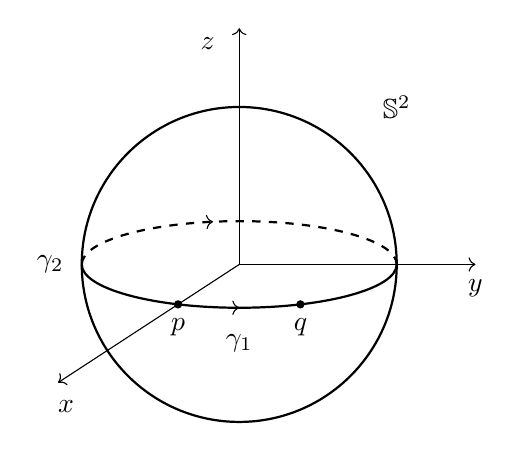
\begin{tikzpicture}[decoration={markings, mark=at position 0.5 with {\arrow{>}}}]
		
		%linee
		\draw [thick] (0,0) circle (2);
		\draw[thick] (-2,0) arc (180:360: 2 and 0.55);
		\draw[decorate] (-2,0) arc (180:360: 2 and 0.55);
		\draw [thick, dashed] (2,0) arc (0:180: 2 and 0.55);
		\draw[decorate] (-2,0) arc (180:42: 2 and 0.55);
		\draw[thin,->] (0,0) -- (0,3);
		\draw[thin,->] (0,0) -- (3,0);
		\draw[thin,->] (0,0) -- (-2.3,-1.5);
		\fill (-0.777,-0.507) circle (1.5pt)
		(0.777,-0.507) circle (1.5pt);
		
		%nomi
		\node at(2,2){\(\Sp^{2}\)};
		\node at (-2.2,-1.8) {\(x\)};
		\node at (3,-0.3){\(y\)};
		\node at (-0.4,2.8){\(z\)};
		\node at  (0,-1) {\(\gamma_1\)};
		\node at  (-2.4,0) {\(\gamma_2\)};
		\node at (-0.777,-0.8){\(p\)};
		\node at (0.777,-0.8) {\(q\)};
		
	\end{tikzpicture}
	
	\caption{\(L(\gamma_1) < L(\gamma_2)\).}
	
	\label{fig: geodetica non minima}
	
\end{figure}
	
	\newpage
	
	Grafico Coseno quadro
	
	\newpage
	
	A¢utointersezione
	
	\newpage
	
	ellissoide
	
	
	
\end{document}